\documentclass[UTF8]{ctexart}
%使用xelatex编译时ctexart会调用xeCJK包自动处理汉字与其它符号的间距
%\usepackage{xeCJK}
%\setCJKmainfont{AR PL UKai CN}

%页面尺寸
\usepackage{geometry}
\geometry{a4paper,centering,scale=0.8}

%增加其他项目到目录中
\usepackage{tocbibind}
%去除目录本身
%\usepackage[nottoc]{tocbibind}

%图表标题
\usepackage[format=hang,font=small,textfont=it]{caption}

%插图功能
\usepackage{graphicx}
\usepackage{float}

%公式引用
\usepackage{amsmath}

%自定义新环境
\newenvironment{myquote}
{\begin{quote}\kaishu\zihao{-5}}
{\end{quote}}

\newtheorem{thm}{定理}

%自定义新命令
\newcommand{\degree}{^\circ}

%参考文件格式
\bibliographystyle{plain}

\title{\heiti 勾股定理}
\author{\kaishu 张三}
\date{\today}


\begin{document}


\maketitle

\begin{abstract}
这是摘要
\end{abstract}

\tableofcontents


\section{第一节}

$90\degree$

参考脚注\footnote{脚注说明}

强调\emph{强调}

\begin{quote}
\zihao{-5}\kaishu 引用 引用 引用 引用 
\end{quote}

\begin{myquote}
自定义引用 引用 引用 引用 
\end{myquote}

\begin{thm}[勾股定理]
这是定理

\end{thm}


数字范围7--8

行内公式$a=b^2$

%列表公式
\begin{equation}\label{eq:gougu}
a^2 + b^2 = c^2 \\
90^{\circ}
\angle ABC = \pi / 2
\end{equation}


\begin{figure}[ht]
\centering
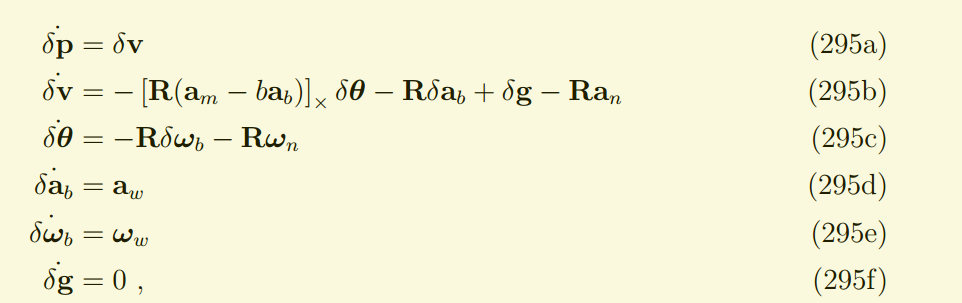
\includegraphics[scale=0.6,width=10cm]{image/test.png}
\caption{插图说明}
\label{fig:xiantu}
\end{figure}

\section{第二节}
下表列出了一些数据:正文和表格直接连一起不浮动[H]
\begin{table}[H]
\begin{tabular}{|rrr|}
\hline
直角边$a$ & 直角边$b$ & 斜边$c$ \\
\hline
3 & 4 & 5 \\
5 & 12 & 13 \\
\hline
\end{tabular}%
\qquad
($a^2 + b^2 = c^2$)
\caption{表格说明}
\label{table:test1}
\end{table}


文献引用\cite{Kline}
文献\cite{quanjing}

插图引用\ref{fig:xiantu} 

表格引用\ref{table:test1}

公式引用 \ref{eq:gougu}

amsmath公式引用 \eqref{eq:gougu} 

 

\nocite{Shiye}
\bibliography{math}

\end{document}